\documentclass[aps,prd,superscriptaddress,groupedaddress,nofootinbib,nobibnotes]{revtex4}

\usepackage{graphicx}
\usepackage{dcolumn}
\usepackage{bm}
\usepackage{amssymb}
\usepackage{epstopdf}
\usepackage{amsmath}
\usepackage{amsfonts}
\usepackage{color}
\usepackage{mathrsfs}
% \usepackage{comment}
% \usepackage{url}
% \usepackage{wick}
% \usepackage{feynmp}
% \usepackage{braket}

\setlength{\parindent}{20pt}
% \setlength{\parskip}{1mm}

\setcounter{topnumber}{1}    % default value is 2.
\setcounter{bottomnumber}{0} % default value is 1.

\hyphenation{ALPGEN}
\hyphenation{EVTGEN}
\hyphenation{PYTHIA}

\newcommand{\kms}[1]{\textcolor{blue}{(KMS: #1)}}
\newcommand{\be}{\begin{equation}}
\newcommand{\ee}{\end{equation}}
\newcommand{\ba}{\begin{eqnarray}}
\newcommand{\ea}{\end{eqnarray}}
\newcommand{\nn}{\nonumber}
\newcommand{\barr}{\begin{array}}
\newcommand{\earr}{\end{array}}
\newcommand{\eqdef}{\stackrel{\rm def}{=}}
\newcommand{\bigoh}{\mathcal{O}}

\newcommand\lsim{\mathrel{\rlap{\lower4pt\hbox{\hskip1pt$\sim$}}
        \raise1pt\hbox{$<$}}}
\newcommand\gsim{\mathrel{\rlap{\lower4pt\hbox{\hskip1pt$\sim$}}
        \raise1pt\hbox{$>$}}}

\def\threej#1#2#3#4#5#6{\left( \begin{array}{ccc} #1 & #2 & #3 \\ #4 & #5 & #6 \end{array} \right) }
\def\smallsum{\mathop{\textstyle\sum}\limits}
\def\Var{\mbox{Var}}
\def\Cov{\mbox{Cov}}

\def\n{{\bf n}}
\def\k{{\bf k}}
\def\x{{\bf x}}
\def\r{{\bf r}}
\def\l{{\bf l}}
\def\th{{\bm{\theta}}}
\def\hr{{\bf \hat r}}
\def\hk{{\bf \hat k}}
\def\tdelta{\tilde\delta}
\def\tf{\tilde f}

\renewcommand{\baselinestretch}{1.1}

\begin{document}

\title{The Limber approximation}

\author{Kendrick~M.~Smith}
\affiliation{Perimeter Institute for Theoretical Physics, Waterloo, ON N2L 2Y5, Canada}

\date{\today}

% \begin{abstract}
% ABSTRACT HERE
% \end{abstract}
% \pacs{}

\maketitle

\section{Setup and notation}

The Limber approximation is a very widely used approximate expression for the
{\em power spectrum $C_l^{ff}$ of a 2D projected field}.  In these notes, we will define 
2D projected fields, state the Limber approximation (Eq.~(\ref{eq:clff_limber}) below),
and give a heuristic derivation.

A 2D projected field is a 2D field which is defined by a line-of-sight
integral of the 3D density field $\delta(\n,\chi)$:
\be
f(\n) = \int d\chi \, W(\chi) \delta(\n\chi, \chi)  \label{eq:los_lightcone}
\ee
The notation here deserves some explanation!
We denote a unit three-vector by $\n$, so that $f(\n)$ is a 2D field defined on the sphere.
We are representing the 3D density field as $\delta(\x, \tau)$, where the first argument $\x$
is a 3D spatial comoving position, with the Earth at $\x=0$.  The second argument $\tau$ is the
``past conformal time'', i.e.~conformal time with $\tau=0$ today, and positive $\tau$ in the past.
Thus, $\delta(\n\chi, \chi)$ denotes the density field evaluated on the past lightcone ($\chi=\tau$), 
where $\chi$ is both the comoving radius and the past conformal time.
The function $W(\chi)$ is a radial weight function which is assumed to be a slowly varying 
function of the comoving radial coordinate $\chi$ (this point will be revisited later).

For examples of cosmologically interesting 2D projected fields, see~\S\ref{sec:examples}.

We would like to compute the power spectrum $C_l^{ff}$ of the 2D field $f$,
in terms of the 3D power spectrum of the density field.  
It turns out that the exact expression for $C_l^{ff}$
is an oscillatory integral in three variables, which is difficult to evaluate numerically and rarely used
(Eq.~(\ref{eq:clff_exact}) below).
The Limber approximation is an approximate expression for $C_l^{ff}$ which is usually very accurate
(1 percent or so) and given by a one-dimensional integral which is well-behaved numerically, and easy
to evaluate.  The Limber approximation is very widely used to compute power spectra of 2D projected fields.

We pause to introduce a little more notation.
Let $\delta(\k,\tau)$ be the Fourier transformed density field, where $\tau$ denotes past conformal time.
By translation and rotation invariance, the two-point function takes the form:
\be
\langle \delta(\k,\tau) \delta(\k',\tau')^* \rangle = P_\delta(k,\tau,\tau') \, (2\pi)^3\delta^3(\k-\k')
\ee
where the {\em unequal-time power spectrum} $P(k,\tau,\tau')$ is defined by this equation.
For the nonlinear density field, this is a function of three variables in principle, but for the linear
density field we can write:
\be
P(k,\tau,\tau') = D(\tau) D(\tau') P(k)  \hspace{1cm} \mbox{(linear theory assumed)}
\ee
Here, $P(k) = P(k,0,0)$ is the matter power spectrum today, and $D(\tau)$ is the
linear growth function.  (Recall that in linear theory, the density field evolves as 
$\delta(\k,\tau) = D(\tau) \delta(\k,0)$, where $D(\tau)$ is the linear growth function.)
We will sometimes write $P(k,\tau) = P(k,\tau,\tau)$ for the equal-time
power spectrum.

Now we give the exact expression for $C_l^{ff}$, which is an oscillatory integral in three
variables, as mentioned above.
\be
C_l^{ff} = \int d\chi \, d\chi' \, \frac{2k^2 \, dk}{\pi} \, W(\chi) W(\chi') j_l(k\chi) j_l(k\chi') P(k,\chi,\chi')  \label{eq:clff_exact}
\ee
where $j_l(x)$ is a spherical Bessel function.  This expression is rarely used, 
but for completeness we give a derivation in Appendix~\ref{app:clff_lightcone}.

The Limber approximation is given by the following one-dimensional integral:
\be
C_l^{ff} \approx \int \frac{d\chi}{\chi^2} \, W(\chi)^2 P(k,\chi)_{k=l/\chi}  \hspace{1cm} \mbox{(Limber approximation)} \label{eq:clff_limber}
\ee
Note that this only involves the equal-time power spectrum $P(k,\tau)$, evaluated at wavenumber $k=l/\chi$
along the past lightcone.

\section{A heuristic derivation of the Limber approximation}
\label{sec:heuristic_derivation}

The 2D projected field $f(\n)$ defined in Eq.~(\ref{eq:los_lightcone}) is 
given by an integral over the past lightcone (Figure~\ref{fig:limber_lightcone}, upper left panel).

Suppose we replace the lightcone geometry by a simplified ``snapshot'' geometry as follows (Figure~\ref{fig:limber_lightcone}, upper right panel).
We pretend that the universe is a 3D periodic box with comoving side lengths ($L_1, L_2, L_3$).
We also take a snapshot of the universe at some past conformal time $\tau_*$.
Thus the density field is a function $\delta(x_1, x_2, x_3)$, where $x_i$ is a comoving spatial coordinate,
and there is no time dependence.
Since we can interpret past conformal time as a comoving radius along the lightcone, we will sometimes write $\chi_*$ for $\tau_*$.

In this snapshot geometry, we construct a 2D projected field $f$ as follows:
\be
f(\theta_1, \theta_2) = \int_0^{L_3} d\chi \, W(\chi_*) \, \delta(\chi_* \theta_1, \chi_* \theta_2, \chi)  \label{eq:los_snapshot}
\ee
In the snapshot geometry, integrating over the 3-axis plays the role of the radial integral in the 
lightcone geometry (Eq.~(\ref{eq:los_lightcone})).
Both the weight function and the density field have been evaluated at a fixed time $\tau=\tau_*$,
unlike the lightcone geometry where they evolve along the lightcone.
In the final 2D projected field $f$, we have rescaled the (1,2) axes, so that $f$ is a function
of ``angular'' coordinates $\theta_i = x_i / \chi_*$.
Thus, $f$ is defined on a flat periodic sky with angular side lengths $(L_1/\theta_*, L_2/\theta_*)$.

In the snapshot geometry, the 2D power spectrum $C_l^{ff}$ is related to the 3D power spectrum $P(k,\tau_*)$ 
in a simple way:
\be
C_l^{ff} = \frac{L_3}{\chi_*^2} W(\chi_*)^2 P(k,\tau_*)_{k=l/\chi_*}
  \hspace{1cm} \mbox{(snapshot geometry)} \label{eq:clff_snapshot}
\ee
where no approximation has been made in deriving this result.
For the derivation of Eq.~(\ref{eq:clff_snapshot}), see Appendix~\ref{app:clff_snapshot}.

Of course, the snapshot geometry is not a very good approximation to the lightcone geometry!
We next define a ``multi-snapshot'' geometry as follows (Figure~\ref{fig:limber_lightcone}, bottom panels).
We assume that the {\em characteristic length scale of variations in the weight function $W(\chi)$ is large compared to the correlation length of the density field}.
(This will turn out to be the criterion for the Limber approximation being an accurate approximation.)

Under this assumption, we can divide the lightcone into slices of comoving thickness $(\Delta\chi)$,
where $(\Delta\chi)$ is chosen to be larger than the correlation length of the density field,
but small enough that the weight function $W$ doesn't evolve much over each slice (Figure~\ref{fig:limber_lightcone}).
Then we can ignore correlations in the density field between slices, and treat each slice as making
an independent contribution to $C_l^{ff}$.
We can also ignore time evolution during the slice, and approximate each slice by the single-snapshot
geometry defined above.
Putting all this together, we get the following expression for $C_l^{ff}$:
\be
C_l^{ff} = \sum \frac{\Delta\chi}{\chi_*^2} W(\chi_*)^2 P(k,\tau_*)_{k=l/\chi_*}
  \hspace{1cm} \mbox{(multi-snapshot geometry)}
\ee
where the sum runs over all slices, and the quantities $(\tau_*, \chi_*)$ are different for each slice.

If we replace this sum by an integral (and change notation $\chi_* \rightarrow \chi$), 
then we get:
\be
C_l^{ff} \approx \int \frac{d\chi}{\chi^2} W(\chi)^2 P(k,\chi_*)_{k=l/\chi_*}
\ee
Note that the dependence on the shell thickness $(\Delta\chi)$ has dropped out.
This agrees with the form of the Limber approximation given previously in Eq.~(\ref{eq:clff_limber}),
and concludes the heuristic derivation.

% Note: Syntax for clipping a figure is
% \includegraphics[trim={5cm 0 0 0},clip,...]
%  where ordering is <left> <lower> <right> <upper>

\begin{figure}
\centerline{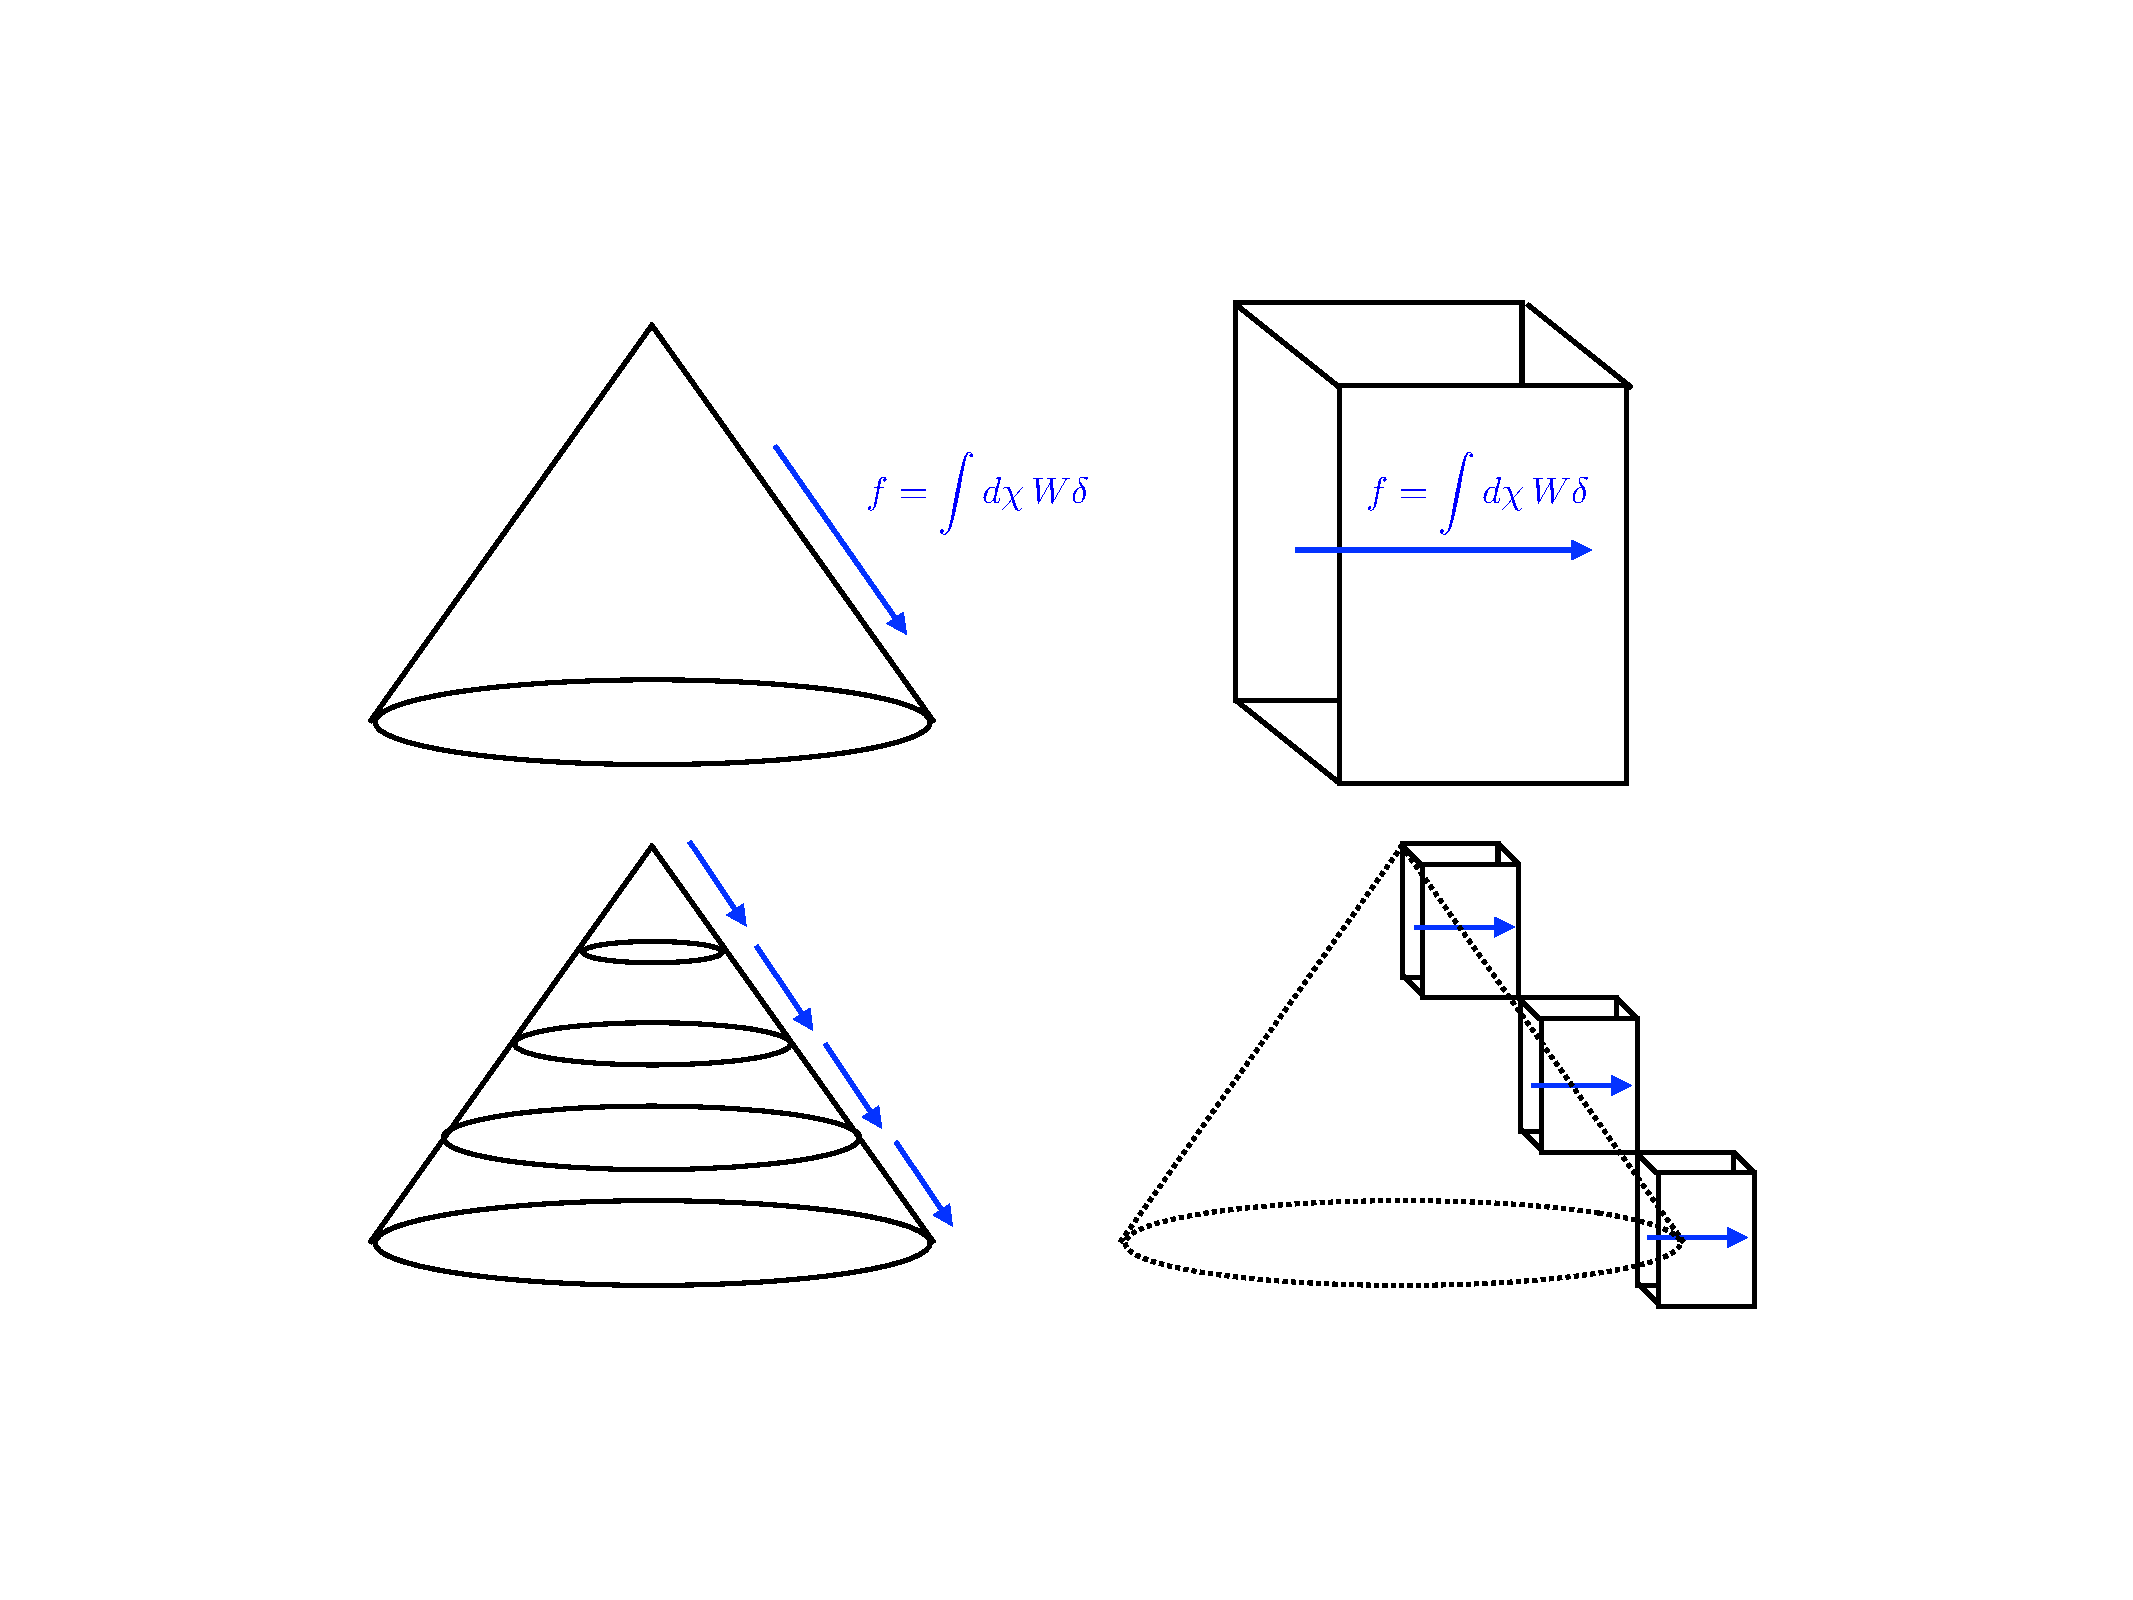
\includegraphics[trim={5cm 5cm 5cm 5cm},clip,width=12cm]{figs/limber_lightcone.pdf}}
\caption{Geometric pictures used in the heuristic derivation of the Limber approximation (\S\ref{sec:heuristic_derivation}).
 {\em Upper left:} Lightcone geometry used to define a 2D projected field (see Eq.~(\ref{eq:los_lightcone})).
 {\em Upper right:} Approximate ``snapshot'' geometry (see Eq.~(\ref{eq:los_snapshot})).
 {\em Bottom panels:} ``Multi-snapshot'' geometry.  We divide the lightcone into shells of width $(\Delta\chi)$,
    then approximate each shell by the snapshot geometry.}
\label{fig:limber_lightcone}
\end{figure}

\section{Examples}
\label{sec:examples}

Here are some interesting special cases of 2D projected fields.

First, consider case of a photometric galaxy survey with redshift distribution $n(z) = dn/dz$
and galaxy bias $b(z)$.  The 2D galaxy overdensity field is:
\be
\delta_g(\n) = \frac{1}{\bar n} \int dz \, n(z) b(z) \delta(\n,z)
\ee
where $\bar n = \int dz \, n(z)$.
Note that this expression neglects Poisson noise, and only represents the clustered part of
the galaxy overdensity field.
To write this as a 2D projected field in standard form (Eq.~(\ref{eq:los_lightcone})), we
change integration variable from $z$ to $\chi$, obtaining:
\be
\delta_g(\n) = \frac{1}{\bar n} \int d\chi \, H(z) n(z) b(z) \delta(\n\chi,\chi)
\ee
This is of the form in Eq.~(\ref{eq:los_lightcone}), with radial weight function:
\be
W(\chi) = \frac{1}{\bar n} H(z) n(z) b(z)
\ee
The Limber approximation is a standard way to compute the 2D angular power spectrum $C_l^{\delta_g\delta_g}$.
(But note that since we have neglected Poisson noise, this will correspond to the 2-halo contribution to
$C_l^{\delta_g\delta_g}$ only.)

Another good example is gravitational lensing.
A full treatment of lensing is beyond the scope of these notes (for a nice review see~\cite{Kilbinger:2014cea}).
Here, we just want to explain how to compute one lensing observable: the convergence field $\kappa(\n)$.
When a population of galaxies is observed, each galaxy may appear magnified or demagnified by large-scale structure
along the line of sight.
It is conventional to write the magnification as $(1 + 2\kappa)$, where the convergence $\kappa$ is defined
by the following line-of-sight integral:
\be
\kappa(\n) = \frac{3 H_0^2 \Omega_m}{2}\int_0^{\chi_0} d\chi \, \frac{\chi(\chi_0-\chi)}{a(\chi) \chi_0} \delta(\n\chi,\chi)
\ee
where $\chi_0$ is the comoving distance to the galaxy being lensed, and $a(\chi)$ is the
scale factor at comoving radius $\chi$.
This is of the form in Eq.~(\ref{eq:los_lightcone}), with radial weight function:
\be
W(\chi) = \left\{ \begin{array}{cl}
   \frac{3 H_0^2 \Omega_m}{2} \frac{\chi(\chi_0-\chi)}{a(\chi) \chi_0} & \mbox{if $\chi \le \chi_0$} \\
     0 & \mbox{if $\chi \ge \chi_0$}
 \end{array} \right.
\ee
In a real lensing survey, the galaxies might be divided into $N$ narrow source redshift bins.
In this case, there would be $N$ convergence fields $\chi_1, \cdots, \chi_N$, corresponding to different values of $\chi_0$.
The Limber approximation could be used to compute the $N$-by-$N$ matrix of power spectra $C_l^{\chi_i \chi_j}$.

\section{Discussion}

Our ``derivation'' of the Limber approximation is heuristic, but I think it gives the most insight into
why it works!  For a formal derivation, see~\cite{LoVerde:2008re}.

So far, we have only considered the case of an auto correlation $C_l^{ff}$, but the Limber approximation
can also be used to calculate cross power spectra.  Suppose that $f(\n)$ and $g(\n)$ are 2D projected fields,
with radial kernels $W_f(\chi)$ and $W_g(\chi)$:
\ba
f(\n) &=& \int d\chi \, W_f(\chi) \delta(\n\chi, \chi) \\
g(\n) &=& \int d\chi \, W_g(\chi) \delta(\n\chi, \chi)
\ea
Then the Limber approximation for the cross spectrum $C_l^{fg}$ is:
\be
C_l^{fg} \approx \int \frac{d\chi}{\chi^2} \, W_f(\chi) W_g(\chi) P(k,\chi)_{k=l/\chi}
\ee

% FIXME: Could add more discussion of the question, how accurate is the Limber approximation?
% FIXME: Sometimes need lower cutoffs on the chi integrals.

% \section*{Acknowledgments}
%
% Research at Perimeter Institute is supported by the Government of Canada
% through Industry Canada and by the Province of Ontario through the Ministry of Research \& Innovation.
% Some computations were performed on the GPC cluster at the SciNet HPC Consortium.
% SciNet is funded by the Canada Foundation for Innovation under the auspices of Compute Canada,
% the Government of Ontario, and the University of Toronto.
% KMS was supported by an NSERC Discovery Grant and an Ontario Early Researcher Award.

\bibliographystyle{h-physrev}
\bibliography{limber_approximation}

\appendix

\section{Exact calculation of $C_l^{ff}$ in lightcone geometry}
\label{app:clff_lightcone}

For reference, in this appendix we derive Eq.~(\ref{eq:clff_exact}) above, which
gives an exact expression for $C_l^{ff}$ as an oscillatory integral in three variables.
We emphasize that the exact expression is rarely used in practice!
Starting from the real-space line-of-sight integral:
\be
f(\n) = \int d\chi \, W(\chi) \delta(\n\chi,\chi)
\ee
we would like to find an analogous Fourier-space expression with $a_{lm}^f$ on the LHS and $\delta(\k,\tau)$
on the RHS.  First we expand $\delta$ in Fourier modes:
\be
f(\n) = \int d\chi \, W(\chi) \int \frac{d^3\k}{(2\pi)^3} \delta(\k,\chi) e^{i\k\cdot(\chi\n)}
\ee
Then we use Rayleigh's expansion, a special function identity which represents a plane wave $e^{i\k\cdot\r}$
in spherical polar coordinates:
\be
e^{i\k\cdot\r} = 4\pi \sum_{lm} i^l j_l(kr) Y_{lm}(\hk)^* Y_{lm}(\hr)
\ee
obtaining:
\be
f(\n) = 4\pi \sum_{lm} i^l \left[ \int d\chi \, \frac{d^3\k}{(2\pi)^3} W(\chi) j_l(k\chi) Y_{lm}(\hk)^* \delta(\k,\chi) \right] Y_{lm}(\n)
\ee
In this form, we can read off $a_{lm}$ (it is the coefficient of $Y_{lm}(\n)$):
\be
a_{lm} = 4\pi i^l \left[ \int d\chi \, \frac{d^3\k}{(2\pi)^3} W(\chi) j_l(k\chi) Y_{lm}(\hk)^* \delta(\k,\chi) \right] Y_{lm}(\n)
\ee
Now we compute the two-point function $\langle a_{lm} a_{l'm'}^* \rangle$:
\be
\langle a_{lm} a_{l'm'}^* \rangle = (4\pi)^2 i^{l-l'} \int d\chi \, d\chi' \, \frac{d^3\k}{(2\pi)^3} \, \frac{d^3\k'}{(2\pi)^3} \,
   W(\chi) W(\chi') j_l(k\chi) j_{l'}(k'\chi') Y_{lm}(\hk)^* Y_{l'm'}(\hk') \, \Big\langle \delta(\k,\chi) \delta(\k',\chi')^* \Big\rangle
\ee
Plugging in $\langle \delta(\k,\chi) \delta(\k',\chi')^* \rangle = P(k,\chi,\chi') \, (2\pi)^3 \delta^3(\k-\k')$, we get:
\be
\langle a_{lm} a_{l'm'}^* \rangle = (4\pi)^2 i^{l-l'} \int d\chi \, d\chi' \, \frac{d^3\k}{(2\pi)^3} \,
   W(\chi) W(\chi') j_l(k\chi) j_{l'}(k\chi') Y_{lm}(\hk)^* Y_{l'm'}(\hk) P(k,\chi,\chi')
\ee
Now we split the $k$-integral into radial and angular parts $\int d^3\k = \int dk \, d^2\hk \, (4\pi k^2)$, and note that the
angular part can be done using the identity (which says that spherical harmonics are orthonormal):
\be
\int d^2\hk \, Y_{lm}(\hk)^* Y_{l'm'}(\hk) = \delta_{ll'} \delta_{mm'}
\ee
This gives:
\be
\langle a_{lm} a_{l'm'}^* \rangle = \left[ \int d\chi \, d\chi' \, \frac{2k^2 \, dk}{\pi} \,
   W(\chi) W(\chi') j_l(k\chi) j_l(k\chi') P(k,\chi,\chi') \right] \delta_{ll'} \delta_{mm'}
\ee
From this expression we can read off the power spectrum:
\be
C_l^{ff} = \int d\chi \, d\chi' \, \frac{2k^2 \, dk}{\pi} \, W(\chi) W(\chi') j_l(k\chi) j_l(k\chi') P(k,\chi,\chi')
\ee
This completes the derivation of Eq.~(\ref{eq:clff_exact}).

\section{Exact calculation of $C_l^{ff}$ in snapshot geometry}
\label{app:clff_snapshot}

In this appendix we derive Eq.~(\ref{eq:clff_snapshot}), which relates the 2D power spectrum $C_l^{ff}$
to the 3D power spectrum $P(k)$ for the simplified ``snapshot'' geometry defined in~\S\ref{sec:heuristic_derivation}.

This is mostly a matter of carefully keeping track of Fourier normalizations,
when translating between fields defined in a periodic box, versus fields defined
in the infinite-volume limit.  In Table~\ref{tab:finite_volume}, we give a
partial ``dictionary'' for translating between the two.  We omit derivations
of the dictionary entries, since a complete discussion would deserve its own
set of notes (but I am happy to talk about it at a blackboard sometime!)

\begin{table}[h!]
\begin{tabular}{|c|c|c|}
\hline
     & Infinite volume  &  Periodic box  \\ \hline
  3D Fourier transform  
      &  $\tdelta(\k) = \int d^3\x \, \delta(\x) e^{-i\k\cdot\x}$
      &  $\tdelta(\k) = \int_0^{L_1} \int_0^{L_2} \int_0^{L_3} d^3\x \, \delta(\k) e^{-i\k\cdot\x}$ \\
  3D inverse Fourier transform  
      &  $\delta(\x) = \int \frac{d^3\k}{(2\pi)^3} \, \tdelta(\k) e^{i\k\cdot\x}$
      &  $\delta(\x) = (L_1L_2L_3)^{-1} \sum_{\k} \tdelta(\k) e^{i\k\cdot\x}$ \\
  3D Power spectrum
      & $\langle \tdelta(\k) \tdelta(\k')^* \rangle = P(k) (2\pi)^3 \delta^3(\k-\k') $
      & $\langle \tdelta(\k) \tdelta(\k')^* \rangle = (L_1L_2L_3) P(k) \delta_{\k\k'}$ \\
  2D Fourier transform  
      &  $\tf(\l) = \int d^2\th \, f(\th) e^{-i\l\cdot\th}$
      &  $\tf(\l) = \int_0^{\theta_1} \int_0^{\theta_2} \, f(\th) e^{-i\l\cdot\th}$ \\
  2D inverse Fourier transform  
      &  $f(\th) = \int \frac{d^2\l}{(2\pi)^2} \, \tf(\l) e^{i\l\cdot\th}$
      &  $f(\th) = (\theta_1\theta_2)^{-1} \sum_{\l} \tf(\l) e^{i\l\cdot\th}$ \\
  2D Power spectrum
      & $\langle \tf(\l) \tf(\l')^* \rangle = C_l (2\pi)^2 \delta^2(\l-\l') $
      & $\langle \tf(\l) \tf(\l')^* \rangle = (\theta_1\theta_2) C_l \delta_{\l\l'}$ \\
\hline
\end{tabular}
\caption{This table gives a dictionary for translating between fields defined in a
  periodic box, versus fields defined in the infinite-volume limit.
  In the ``periodic box'' column, we assume that 3D fields are defined in a box with 
  comoving side lengths $(L_1,L_2,L_3)$, and 2D fields are defined on a periodic flat sky
  with angular side lengths $(\theta_1,\theta_2)$.
  In the ``infinite volume'' column, we assume that 3D fields are defined in an infinite
  comoving volume, and 2D fields are defined on an infinite {\em flat} sky.}
\label{tab:finite_volume}
\end{table}

Armed with this dictionary, we derive Eq.~(\ref{eq:clff_snapshot}) as follows.
First, we work out the relation between Fourier modes $f(\l)$ of the 2D projected field,
and Fourier modes $\delta(\k)$ of the 3D density field.
\ba
f(\l)
  &=& \int_0^{\theta_1} \int_0^{\theta_2} d^2\th \, f(\theta_1,\theta_2) e^{-i\l\cdot\th} \nn \\
  &=& \int_0^{\theta_1} \int_0^{\theta_2} d^2\th \, \int_0^{L_3} d\chi \, W(\chi_*) \delta(\chi_*\theta_1, \chi_*\theta_2, \chi) e^{-i\l\cdot\th} \nn \\
  &=& \chi_*^{-2} \int_0^{L_1} \int_0^{L_2} \int_0^{L_3} dx_1 \, dx_2 \, dx_3 \, W(\chi_*) \delta(x_1, x_2, x_3) e^{-i(l_1 x_1 + l_2 x_2) / \chi_*} \nn \\
  &=& \frac{1}{\chi_*^2} W(\chi_*) \, \tdelta\!\left( \frac{l_1}{\chi_*}, \frac{l_2}{\chi_*}, 0 \right) 
\ea
In the first line, we have used the fourth entry in the dictionary (``2D Fourier transform'').
In the second line, we have used the definition of $f$ (Eq.~(\ref{eq:los_snapshot})).
In the third line, we have changed integration variable $x_i = \chi_* \theta_i$, and renamed $\chi \rightarrow x_3$.
Note that $L_1 = \chi_* \theta_1$ and $L_2 = \chi_* \theta_2$.
In the fourth line, we have used the first entry in the dictionary (``3D Fourier transform'')
to recognize the result as $\tdelta(\k)$ evaluated at wavenumber $\k = (l_1/\chi_*, l_2/\chi_*, 0)$.

Using this result, we compute the two-point function $\langle \tf(\l) \tf(\l')^* \rangle$:
\ba
\langle \tf(\l) \tf(\l')^* \rangle
  &=& \frac{1}{\chi_*^4} W(\chi_*)^2 \left\langle 
      \, \tdelta\!\left( \frac{l_1}{\chi_*}, \frac{l_2}{\chi_*}, 0 \right) 
      \, \tdelta\!\left( \frac{l_1'}{\chi_*}, \frac{l_2'}{\chi_*}, 0 \right)^*
   \right\rangle \nn \\
  &=& \frac{1}{\chi_*^4} W(\chi_*)^2 (L_1L_2L_3) P(k,\chi_*)_{k=l/\chi_*} \delta_{\l\l'} \nn \\
  &=& \frac{L_3}{\chi_*^2} W(\chi_*)^2 (\theta_1\theta_2) P(k,\chi_*)_{k=l/\chi_*} \delta_{\l\l'}
\ea
In the second line, we have used the third entry in the dictionary (``3D power spectrum'').
In the third line, we have written $L_1 = \chi_* \theta_1$ and $L_2 = \chi_* \theta_2$.

Now, using the last entry in the dictionary (``2D power spectrum''), we can read off $C_l^{ff}$:
\be
C_l^{ff} = \frac{L_3}{\chi_*^2} W(\chi_*)^2 P(k,\chi_*)_{k=l/\chi_*}
\ee
This completes the derivation of Eq.~(\ref{eq:clff_snapshot}).

\end{document}
